\documentclass[10pt, blue,subsection=true, compress]{beamer}
%\documentclass{powerdot}
%\documentclass[compress, red]{beamer}
\usetheme{Warsaw}                            % Beamer Theme
\usecolortheme{lily}                         % Beamer Color Theme
\useoutertheme[subsection=true]{smoothbars} % Beamer Outer Theme
\useinnertheme{rounded}                   % Beamer Inner Theme
\mode<presentation>
%\usetheme{Copenhagen} 
\usepackage{graphicx}
\usepackage{amsthm}
\usepackage{amsmath}    % for math AMS fonts
\usepackage{graphicx}   % to include figures
\usepackage{subfigure}   % to have figures in figures
\usepackage{multimedia} % to include movies
\usepackage{epsfig}
%\setbeamercovered{transparent}
%\usefonttheme[onlymath]{serif}
%\usepackage{hyperref}
%\pdfoutput=1
\hypersetup{pdfstartview={FitB}}
%\hypersetup{pdfstartview={XYZ null null 1.00}} % By default the pdf fit the width of the screen.
 \usepackage[usenames,dvipsnames]{pstricks}
 %\usepackage{epsfig}
 \usepackage{pst-grad} % For gradients
 \usepackage{pst-plot} % For axes
 \DeclareMathOperator*{\argmax}{arg\,max}
   
% USE FILE %%%%%%%%%%%%%%%%%%%%%%%%%%%%%%%%%%%%%%%%%%%%%%%%%%%%%%%%

%%%%%%%%%%%%%%%%%%%%%%%%%%%%%%%%%%%%%%%%%%%%%%%%%%%%%%%%%%%%%%%%%%%%%%%%%%%%%%%%%%%%%%%%%%%%%%%%%

\title[Second Order Pseudolikelihood Learning in Relational Domain]{Second Order Pseudolikelihood Learning in Relational Domain }

\author[Krishna Kumar Tiwari]{Krishna Kumar Tiwari \newline Under the guidance of Dr.V. Vijaya Saradhi}


\institute[IITG]{Department of Computer Science\\ Indian Institute Of Technology Guwahati\\[1ex]
\texttt{k.tiwari@iitg.ernet.in} }

\date[July 2011]{July 7, 2011}

%%%%%%%%%%%%%%%%%%%%%%%%%%%%%%%%%%%%%%%%%%%%%%%%%%%%%%%%%%%%%%%%%%%%%%%%%
\begin{document}

\begin{frame}
  \titlepage
\end{frame}
%%%%%%%%%%%%%%%%%%%%%%%%%%%%%%%%%%%%%%%%%%%%%%%%%%%%%%%%%%%%%%%%%%%%%%%%%%%%%%%%
\section[Outline]{}
%\subsection {}
% Creates table of contents slide incorporating
% all \section and \subsection commands
\begin{frame}
  \tableofcontents
 
\end{frame}

%----------------------------------------------------------------------------------------------------------

\section{Introduction}
%%%%%%%%%%%%%%%%%%%%%%%%%%%%%%%%%%%%%%%%%%%%%%%%%%%%%%%%%%%%%%%%%%%%%%%%%%%%%%%%%%%%%%%
%--------------------------------------------------------------------

\begin{frame} \frametitle{Traditional Vs. Relational Learning}

\begin{columns}[t]
\column{0.3\textwidth} 
\begin{flushleft}
\begin{block} {Traditional Domain}\
\begin{itemize}
\item Instances follows \textit{i.i.d} assumption.
\item Homogeneous objects. 
\end{itemize}

\end{block}
\end{flushleft}

\column{0.3\textwidth}
 
\begin{flushleft}
\begin{block} {Statistical Relational Learning}
\begin{itemize}
\item Violates \textit{i.i.d} assumption.
\item Heterogeneous objects and links.
\end{itemize}
\end{block}
\end{flushleft}

\column{0.3\textwidth}
 
\begin{flushleft}
\begin{block} {Real World Data}
\begin{itemize}
\item Structured, Semi structured, Unstructured.
\item Heterogeneous objects and links.
\end{itemize}
\end{block}
\end{flushleft}
\end{columns}


\begin{columns}[t]
\column{0.4\textwidth} 
\begin{flushleft}
\begin{block}{Citation Database}
\scalebox{.3} % Change this value to rescale the drawing.
{
\begin{pspicture}(0,-2.5)(7.6,2.5)
\rput(3.8,2.5){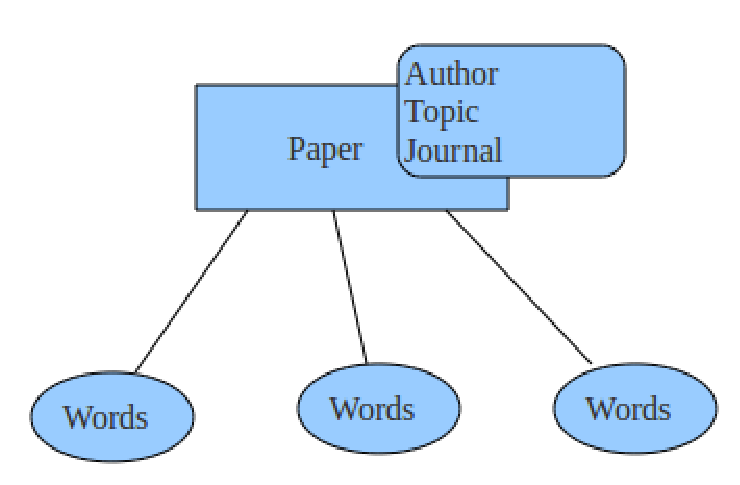
\includegraphics{/home/krishna/Desktop/Final7/shadi/img/bags.eps}}
\end{pspicture} 
}

\end{block}
\end{flushleft}
\column{0.4\textwidth} 
\begin{block}{Examples}
citation database (HEP), Movie database (IMDB), 
Hypertext classification database (ProxWebKB)
\end{block}
\end{columns}
\end{frame} 




\begin{frame} \frametitle{Relational Learning Opportunities}
\begin{itemize}
\item \textbf{Object Classification --} Example, in citation database, predicting
the topic of a paper. 
\item \textbf{Object Type Prediction--} Predict whether a set of pages belong to 
conference paper, master's thesis or technical report.
\item \textbf{Link Type Prediction--} Predicting a paper is published in journal, conference or
workshop. 
\item \textbf{Predicting Link Existence--} Given two papers are related or not.
\item \textbf{Link Cardinality Estimation--} Predicting the number of citations of a paper.
\item \textbf{Group Detection--} In movie database, identifying groups of same type of
movies.
\end{itemize}

\end{frame} 

\begin{frame} \frametitle{Challenges}
\begin{block} {\textbf{How to model relational data ?}} 
\begin{itemize}
\item Represent as graphs.
\item Represent in multiple tables.
\item Represent in terms of fist order logic statements.
\end{itemize}
\end{block}

\begin{block}{\textbf{Individual vs. Collective classification}} 
\begin{itemize}
\item Individual classifiers assumes class label of related entities are independent.
\item Collection classification uses related entities class label along with other attribute.
\end{itemize}
\end{block}

\begin{block}{\textbf{Logical vs. Statistical dependencies}}
\begin{itemize}
\item Logical : $A \rightarrow B$
\item Statistical : $Correlation (A,B) = 0.6$
\end{itemize}
\end{block}
\end{frame} 

% Section graphical Models
\section{Graphical Models}
\begin{frame} \frametitle{Graphical Models}
\begin{columns}[t]
\column{0.5\textwidth} 
\begin{flushleft}
\begin{block}{Directed Models}
\begin{itemize}
\item Does not allow cyclic dependencies among the attributes.
\item Simple parameter estimation and structure learning technique.
\item Relational Bayesian Networks. 
\end{itemize}
\end{block}
\end{flushleft}
\column{0.5\textwidth} 
\begin{block}{Bayesian Networks}
\begin{figure}[htbp]
\centering
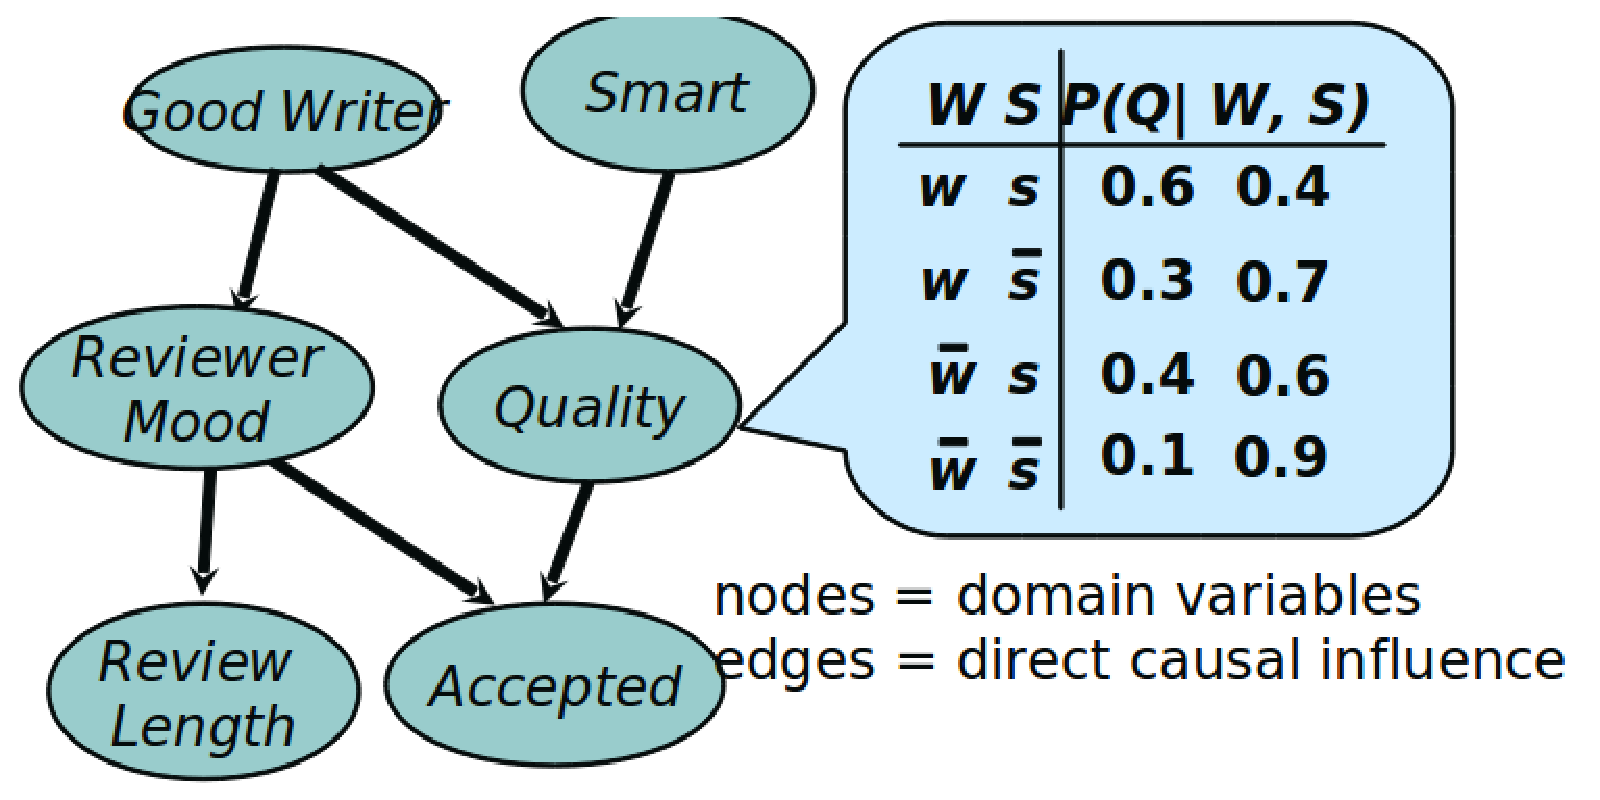
\includegraphics[scale=0.2]{/home/krishna/Desktop/Final7/shadi/img/rbn.eps}
\end{figure}
\end{block}
\end{columns}
\end{frame} 

\begin{frame}\frametitle{Graphical Models}
\begin{columns}[t]
\column{0.5\textwidth} 
\begin{flushleft}
\begin{block}{Undirected Models}
\begin{itemize}
\item Represent cyclic dependencies. 
\item Requires known network structure.
 \item Parameter estimation requires repeated inference over large values.
 \item Relational Markov Networks.
\end{itemize}
\end{block}
\end{flushleft}
\column{0.5\textwidth} 
\begin{block}{Markov Networks}
\begin{figure}[htbp]
\centering
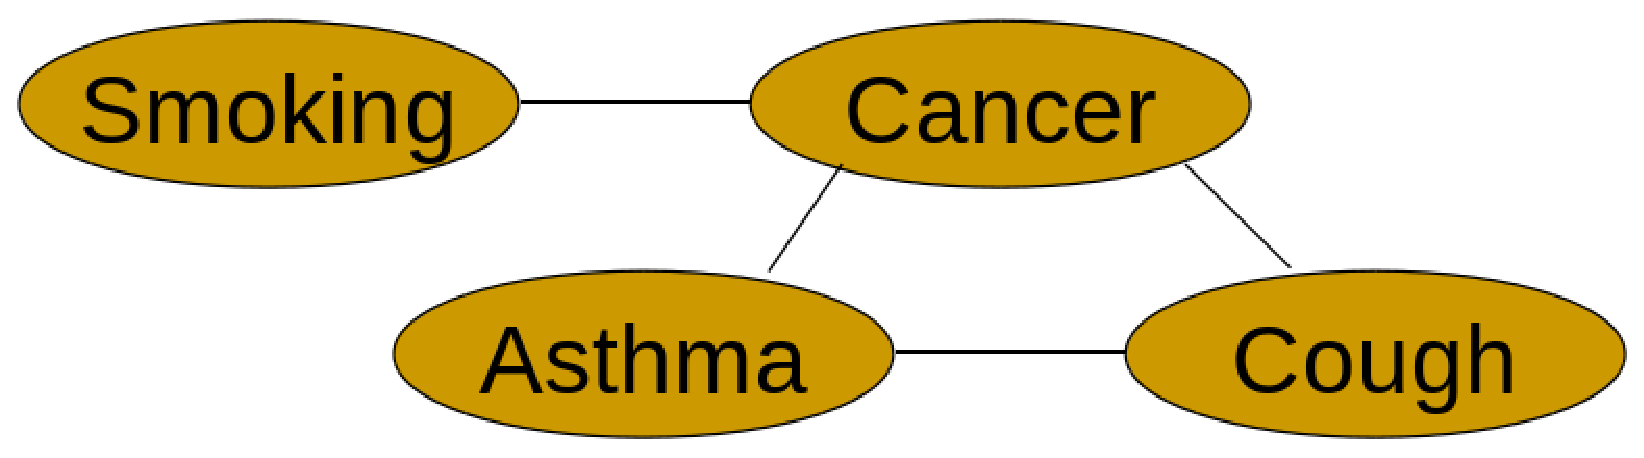
\includegraphics[scale=0.2]{/home/krishna/Desktop/Final7/shadi/img/rmn.eps}
\end{figure}
\end{block}
\end{columns}
\begin{center}
\begin{block}{{\color{red} Relational Dependency Networks}}
\begin{itemize}
\item Approximate model.
\item First model to learn autocorrelation. 
\item Simple structure learning and parameter estimation.
\end{itemize}
\end{block}
\end{center}
\end{frame}
% Approximation Methods.
\section{Approximation Methods}
\begin{frame}\frametitle{Approximation Methods}
\begin{block}{}
 Assume data contains n samples of m dimensional vectors 
following \textit{i.i.d}, sampled from a distribution 
$p_{\theta_{0}}$ with $\theta_{0} ~ \in ~\Theta ~ \subset R^r $,
\begin{equation*}
 D = (X^1,.....X^n ),  \: \hspace{3mm}   X^i  ~\in ~ R^m ,
\end{equation*}
\end{block}


\begin{columns}[t]
\column{0.5\textwidth} 
\begin{flushleft}
\begin{block}{\textbf{Maximum likelihood estimator}} 
MLE is defined as:
\begin{align}
 l_n(\theta ; D) = \sum_{i=1}^n p_{\theta}(X^i)\\
\nonumber {\widehat{\theta}^{ml}}_n  =  \argmax_{\theta_{0} ~\in~ \theta}  l_n (\theta ; D)
\end{align}

\end{block}
\end{flushleft}
\column{0.5\textwidth} 
\begin{block}{ \textbf{Pseudolikelihood}}
PL is defined as:
\begin{align}
pl_n (\theta ; D) = \sum_{i=1}^n \sum_{j=1}^m log
p_{\theta}({X^i_j} | {X^i_{-j}}). 
\end{align}
Where subscript represents dimension and $X_{-j}^i = \{ X_k^i ~: k \neq j\}$.
\end{block}
\end{columns}
\end{frame}


\begin{frame}\frametitle{Approximation Methods}
\begin{block}{\textbf{Composite Likelihood}}
\begin{itemize}
\item Composite likelihood is a generalization of pseudolikelihood function.
\item Composite likelihood function  is defined as :
\begin{equation}
\label{comp}
 cl_n = \sum_{i=1}^n \sum_{j=1}^k log p_{\theta}(X_{A_j}^i | X_{{B_j}}^i). 
\end{equation}
$A \neq \emptyset = A \cap B$, 
where A and B represents the dimension set of the instance X.  
\item If $|A_i| =1$ then composite likelihood represents pseudolikelihood. 
\item Dillon extended composite likelihood by introducing component weight and selection probabilities to make it stochastic composite likelihood.
\item Variance of the model is minimum in case of full likelihood and maximum in pseudolikelihood.
\end{itemize}
\end{block}

% Add a comparison chart 
\end{frame}

% Relational Dependency Networks
\section{Relational Dependency Networks}
\begin{frame}\frametitle{Relational Dependency Networks}
\textbf{Data Graph}
$G_D = (V_D , E_D)$. $V_D$ represents objects in the data graph and $E_D$ represents relationship between these objects.
\begin{figure}[htbp]
\centering
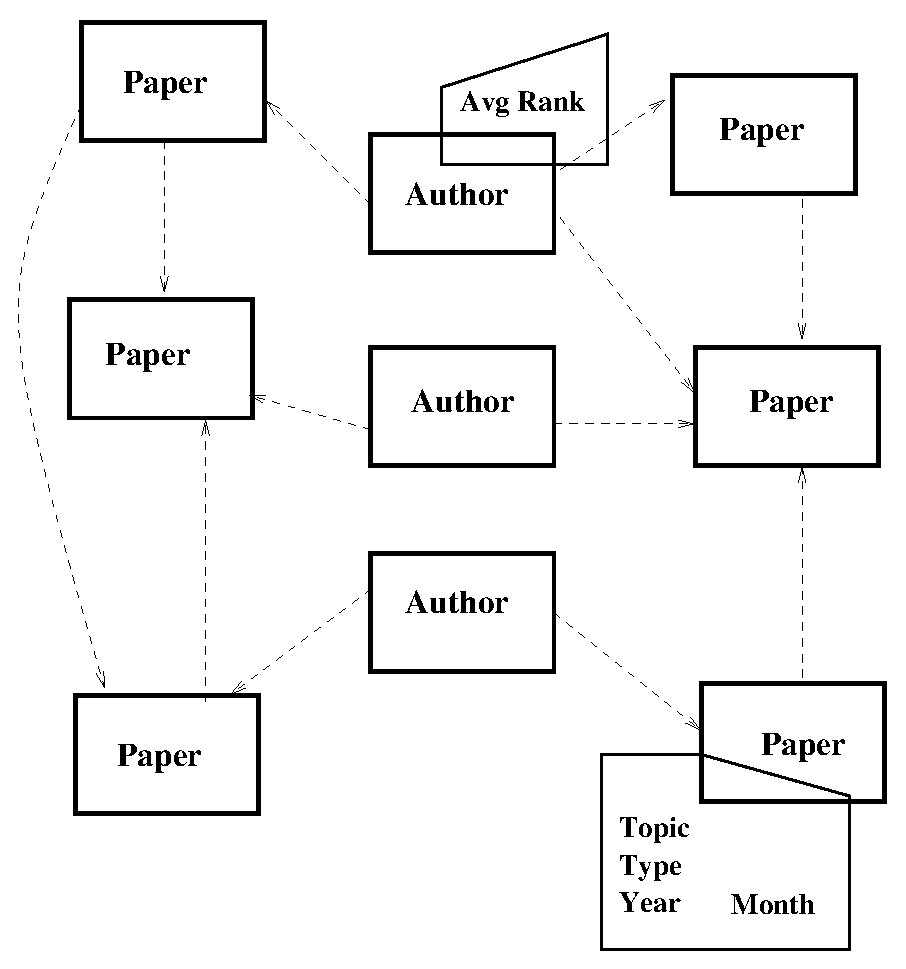
\includegraphics[scale=0.2]{/home/krishna/Desktop/Final7/shadi/img/data.eps}
\caption{Data Graph}
\label{fig:3.2}
\end{figure}
RDN represents a joint distribution over the values of the attributes in the data graph, 
\begin{align}
\nonumber  x = \left\{\{X_{v_i}^{t_{v_i}} : v_i \in V~ s.t. ~T(v_i) = t_{v_i}\}  \cup \{X_{e_j}^{t_{e_j}} : e_j \in E ~s.t.~ T(e_j) = t_{e_j} \}\right\}
\end{align}



\end{frame}

\begin{frame}

Approximation of $p(x)$ is done by pseudolikelihood to learn the parameters.
\begin{align}
\label{plgd}
  PL( G_D; \theta)= \prod_{t \in T} \prod_{X^t_i \in X^t} \prod_{v : T ( v) =t } p(x^t_{v_i} | pa_{x^t_{v_i}} ; \theta ) 
\prod_{e :T( e) =t} p( x^t_{e_i} | pa_{x^t_{e_i}} ; \theta)
\end{align}
 \textbf{Model Graph} $G_M = (V_M, E_M)$ represents probabilistic relationship between the attributes.
\begin{figure}[htbp]
\centering
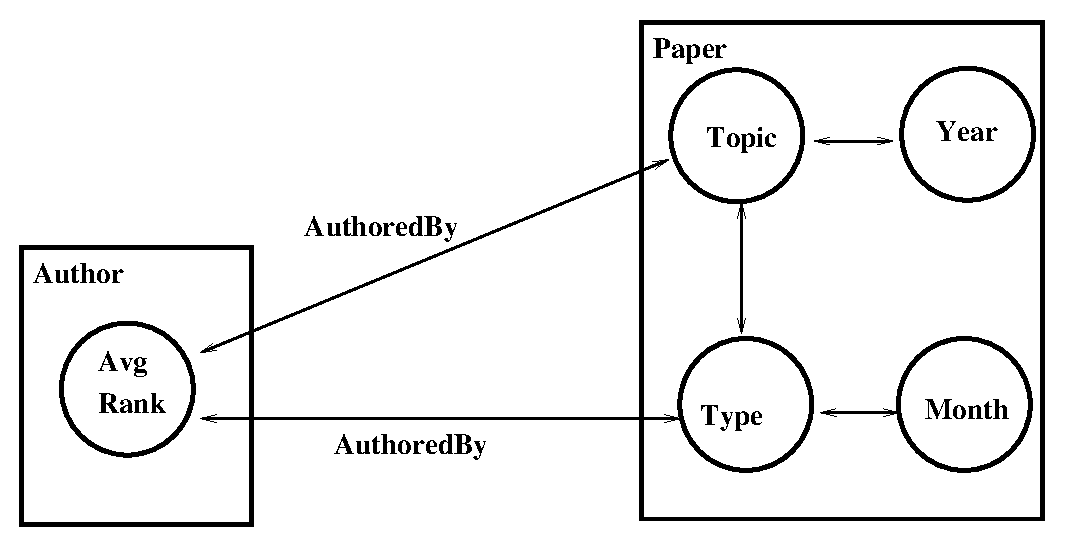
\includegraphics[scale=0.2]{/home/krishna/Desktop/Final7/shadi/img/model.eps}
\caption{Model Graph}
\label{fig:3.2}
\end{figure}
 RDN uses relational learners to learn CPDs.
\begin{itemize}
\item {\color{red}Relational Bayesian Classifier (RBC)}
\item Relational Probability Tree (RPT)
\end{itemize}
\end{frame}
\begin{frame}\frametitle{Relational Bayesian Classifier}
\begin{itemize}
\item Treats heterogeneous subgraphs as a homogeneous set of attributes multisets.
\item Deals with multisets of different sizes. Ex. In case of citation database, considering publication dates of cited papers form multisets of varying size (e.g. 
\{2002,2002,2006,2009\}, \{2004,2007,2009\}). 
\begin{columns}[t]
\column{0.5\textwidth} 
\begin{block}{Relational data representation}
\begin{figure}[htbp]
\centering
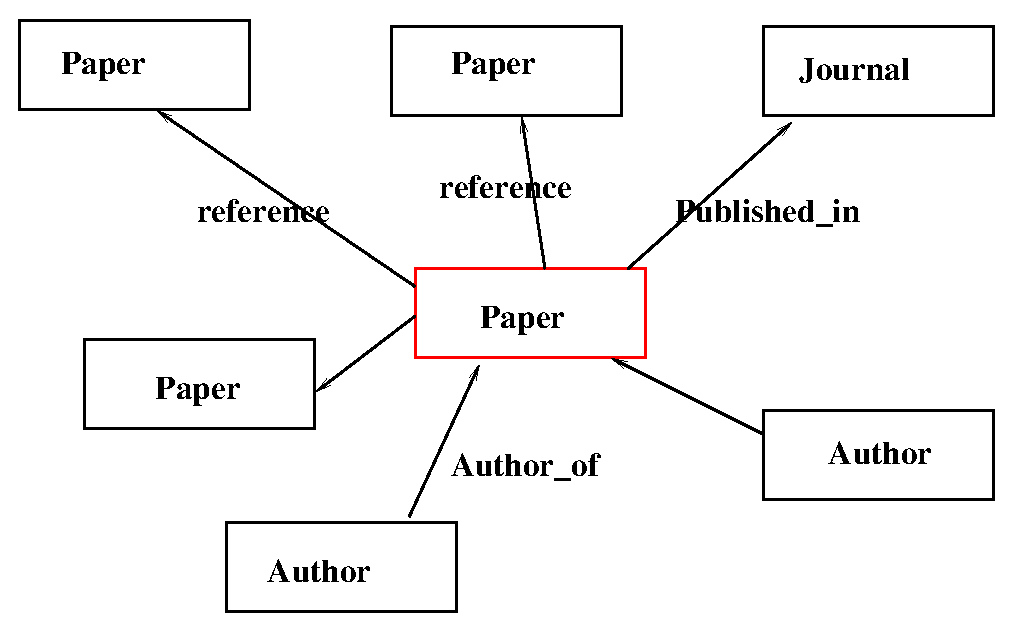
\includegraphics[scale=0.2]{/home/krishna/Desktop/Final7/shadi/img/rbc.eps}
\end{figure}
\end{block}
\column{0.5\textwidth} 
\begin{block}{Homogeneous attribute representation}
\begin{figure}[htbp]
\centering
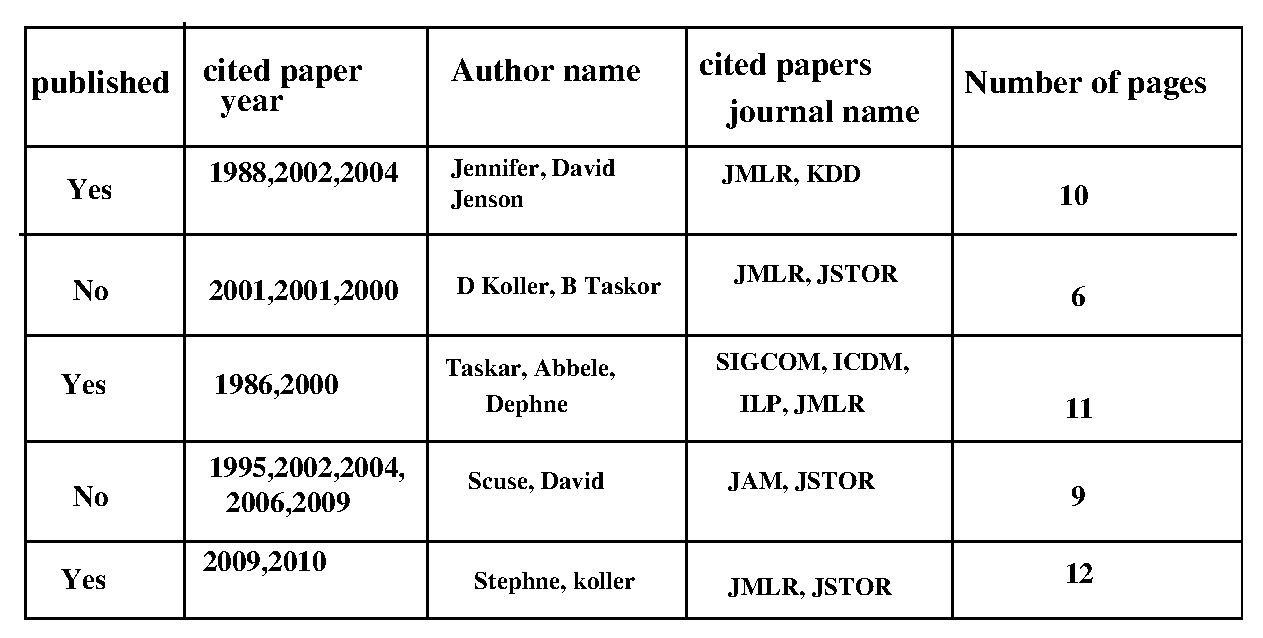
\includegraphics[scale=0.2]{/home/krishna/Desktop/Final7/shadi/img/rbc2.eps}
\end{figure}
\end{block}
\end{columns}
\item Independent assumption among the values of set performs best. 
\end{itemize}
\end{frame}

% Second Order PL in RDN
\section{Second Order PL in RDN}
\begin{frame}\frametitle{Second Order PL in RDN}
\begin{block}{\textbf{Motivation}}
\begin{itemize}
\item Choice of different order of likelihood object gives us different ways to approximate joint distribution $p(x)$.
\item In highly correlated environment it is better to deal with appropriate combination of attribute. 
\end{itemize}
\end{block}
We define composite likelihood in RDN as :
 \begin{align}
\label{eq:clgd}
 cl(G_D ; \theta)  =  \prod_{t  \in  T} \prod_{ X_{A_i}^t  \in X^t}^k \prod_{ v: T(v) = t } p ( x^t_{v_{A_i}} | pa_{ x^t_{v_{B_i}}}) 
 \prod_{ e :T(e) = t } p ( x^t_{e_{A_i}}  | pa_{ x^t_{e_{B_i}}}) 
\end{align}
\begin{align*}
 \intertext{Subject to the constraint:}
  \nonumber   A_i \neq \emptyset = A_i \cap B_i 
\end{align*}
Where $A_i$ and $B_i$ represents set of dimensions.
\end{frame}

\begin{frame}\frametitle{Second Order PL in RDN}
We are denoting second order pseudolikelihood as $pl_2(G_D ; \theta)$.
\begin{align} 
 pl_2(G_D ; \theta) = \sum_{t \in T} \sum_{X_{\{p,q\}}^t \in X^t}^k \sum_{v: T(v) = t} p (x^t_{v_{A_i}} | pa_{x^t_{v_{B_i}}}) 
\sum_{e :T(e) = t} p (x^t_{e_{A_i}} | pa_{x^t_{e_{B_i}}})
\end{align}
\begin{block}{Comparison with PL}
\begin{itemize}
\item Generalization of PL in the context of RDN.
\item Second order PL deals with pair of attributes.
\end{itemize}
\end{block}
\begin{block}{}
\begin{center}
\textbf{\color{red}
Second Order Relational Learners?}
\end{center}
\end{block}
\end{frame}


% Second Order RBC

\section{Second Order RBC}
\begin{frame}\frametitle{Second Order RBC}
\begin{itemize}
\item  Initially we have set of attributes denoted as $A = \{ X_1, X_2, \cdots, X_m\}$. 
\item Second order RBC makes all possible pair of attributes and denoted as \textit{P}.
\begin{align*}
 P = \{ \{ X_1, X_2\}, \{ X_1, X_3\}, \cdots, \{ X_{m-1}, X_m\}\} \\
\end{align*}
\item Second order RBC select elements from \textit{P} which lead to the full likelihood denoted as set \textit{S}. 
\begin{block}{Definition of set \textit{S}}
\begin{align}
\label{eq:s}
    S = \{ s_i ~: s_i \in P  \}\\
   \text{Subject to the constraints:} \notag \\
   \nonumber \tag{7.a} \forall~ s_i, s_j ~ \in ~S ~~ s_i \cap s_j ~ = \emptyset \\
   \nonumber \tag{7.b} \displaystyle{\cup_{i=1}^{|S|}} ~ s_i = A 
\end{align}
\end{block}
\end{itemize}
\end{frame}

\begin{frame}\frametitle{Construction of set \textit{S}}
\begin{figure}[htbp]
\centering
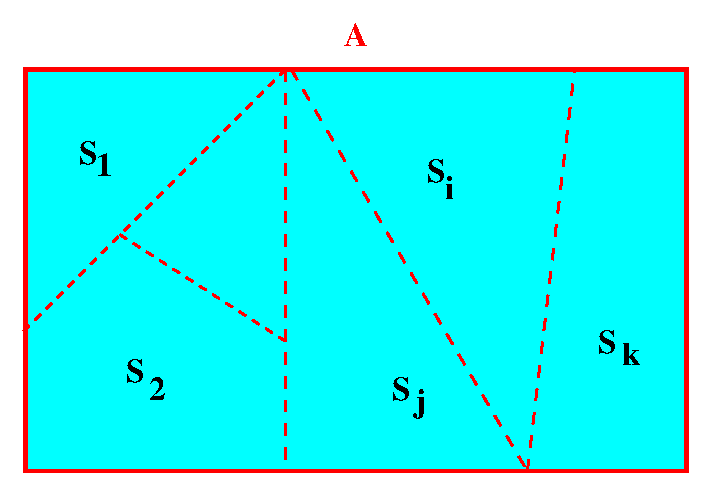
\includegraphics[scale=0.2]{/home/krishna/Desktop/Final7/shadi/img/s.eps}
\end{figure}
\begin{block}{\textbf{Exhaustive Search}}
Choose the subset from \textit{P} which maximize the likelihood of the class.
\begin{align}
S \equiv \argmax_{p ~ \subsetneq ~ P} ~  P(C | p)
\end{align}
\end{block}

\begin{block}{\textbf{Greedy Approach}}
\begin{itemize}
\item Assign score to all elements of set \textit{P}.
\begin{align}
 score(p_i) = log P( C | p_i ~\in~ P) ~\equiv ~ log P( C | \{X_i,X_j\}) 
\end{align}
\item Add maximum score elements of \textit{P} to \textit{S} by maintaining the constraints of equation \eqref{eq:s}.
\end{itemize}
\end{block}
\end{frame}

\begin{frame}\frametitle{Second Order PL in RBC}
\begin{block}{Second Order PL in RBC}
According to modified second order PL,  
\begin{align}
\nonumber
 P(C | \{a_1,a_2,....a_m\}) ~ \propto ~ P(A | C)*P(C) \\
\equiv P(S | C)*P(C)=  \prod_{i=1}^{|S|} ~ P(s_i | C)*P(C)
\end{align}
\end{block}
\begin{block}{Complexity Analysis}
Second order RBC learning has three major components. 
\begin{itemize}
 \item Assignment of score to all elements of set \textit{P}, it takes $O(|P|\times N)$, where N is number of subgraphs.
\item Sorting of the scores, it takes $O(|P| \times log(|P|)$. 
\item Construction of set \textit{S} takes $O(|P|^2)$
\end{itemize}
Overall \emph{asymptotic} complexity of second order RBC is $O(|P|\times N)$.
\end{block}
\end{frame}

% Experimental Results
\section{Experimental Results}
\begin{frame}\frametitle{Synthetic Data Results}
\begin{block}{QGraph Query}
\begin{figure}[htbp]
\centering
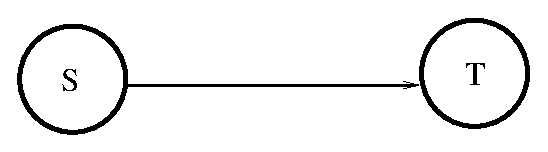
\includegraphics[scale=0.3]{/home/krishna/Desktop/Final7/shadi/img/container1d.eps}
\end{figure}
\end{block}
\begin{columns}[t]
\column{0.5\textwidth} 
\begin{block}{Accuracy Comparison}
\begin{figure}[htbp]
\centering
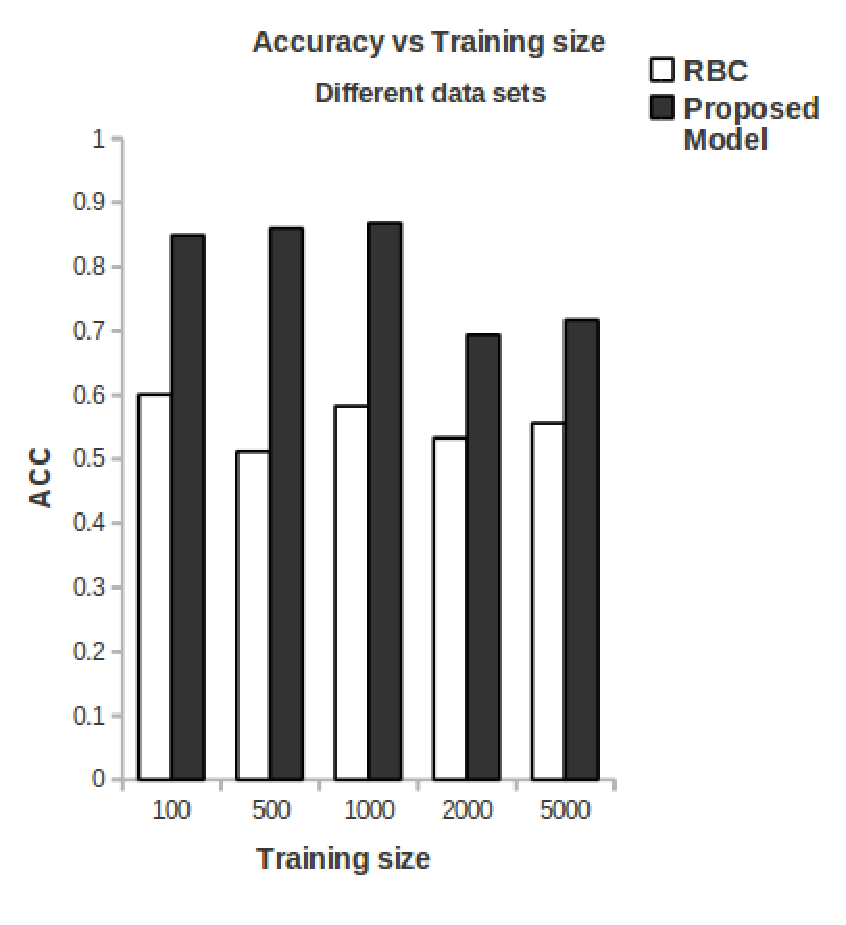
\includegraphics[scale=0.25]{/home/krishna/Desktop/Final7/shadi/img/ex1-acc.eps}
\end{figure}
\end{block}
\column{0.5\textwidth} 
\begin{block}{Likelihood Comparison}
\begin{figure}[htbp]
\centering
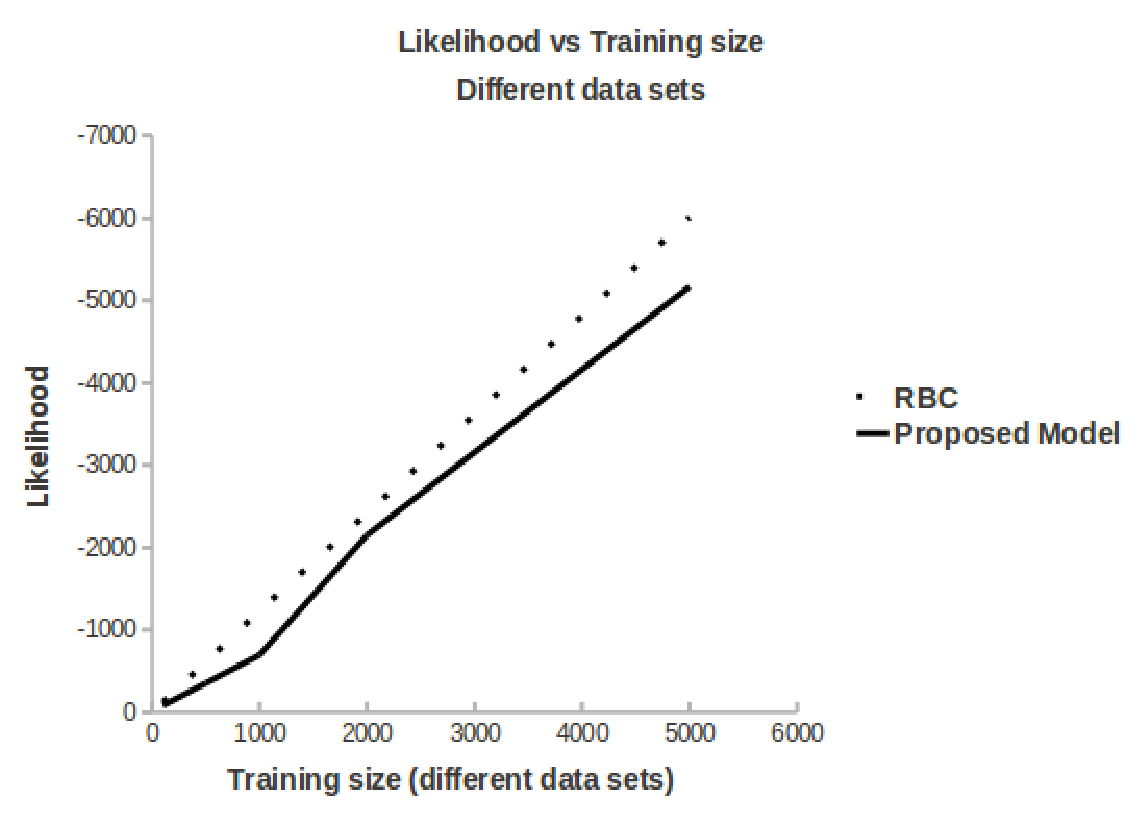
\includegraphics[scale=0.25]{/home/krishna/Desktop/Final7/shadi/img/ex1-lh.eps}
\label{fig:4.2}
\end{figure}
\end{block}
\end{columns}
\end{frame}
\begin{frame}\frametitle{Synthetic Data Results}
\begin{block}{QGraph Query}
\begin{figure}[htbp]
\centering
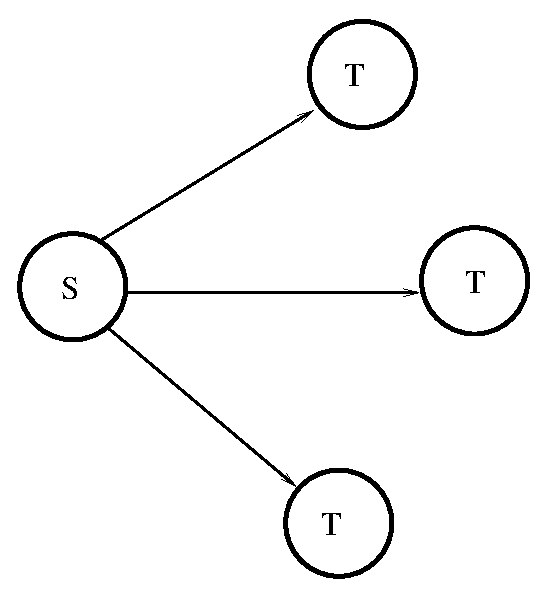
\includegraphics[scale=0.15]{/home/krishna/Desktop/Final7/shadi/img/container2d.eps}
\end{figure}
\end{block}
\begin{columns}[t]
\column{0.5\textwidth} 
\begin{block}{Accuracy Comparison}
\begin{figure}[htbp]
\centering
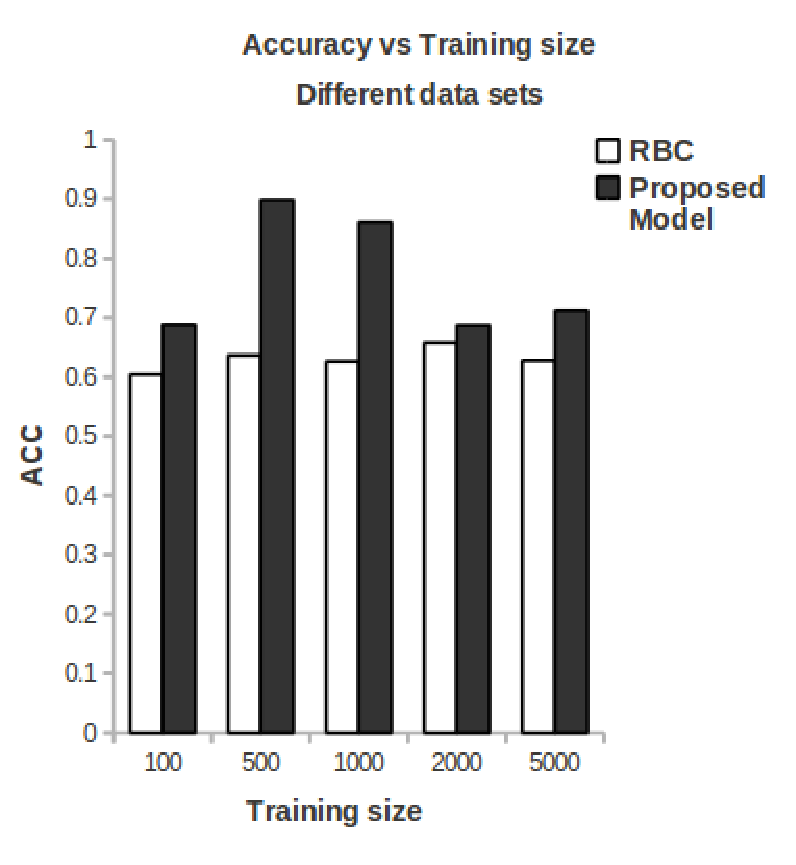
\includegraphics[scale=0.25]{/home/krishna/Desktop/Final7/shadi/img/ex2-acc.eps}
\end{figure}
\end{block}
\column{0.5\textwidth} 
\begin{block}{Likelihood Comparison}
\begin{figure}[htbp]
\centering
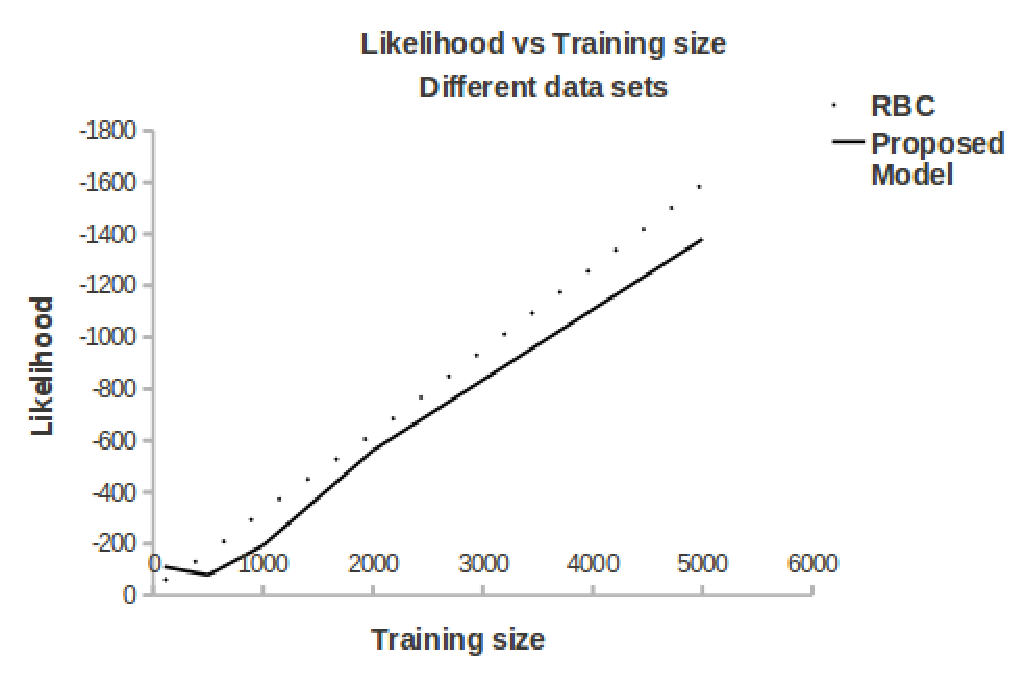
\includegraphics[scale=0.25]{/home/krishna/Desktop/Final7/shadi/img/ex2-lh.eps}
\label{fig:4.2}
\end{figure}
\end{block}
\end{columns}
\end{frame}
\begin{frame}\frametitle{Synthetic Data Results}
\begin{itemize}
\item \textbf{Effect of Correlation}
\begin{columns}[t]
\column{0.5\textwidth} 
\begin{block}{Accuracy vs. Correlation}
\begin{figure}[htbp]
\centering
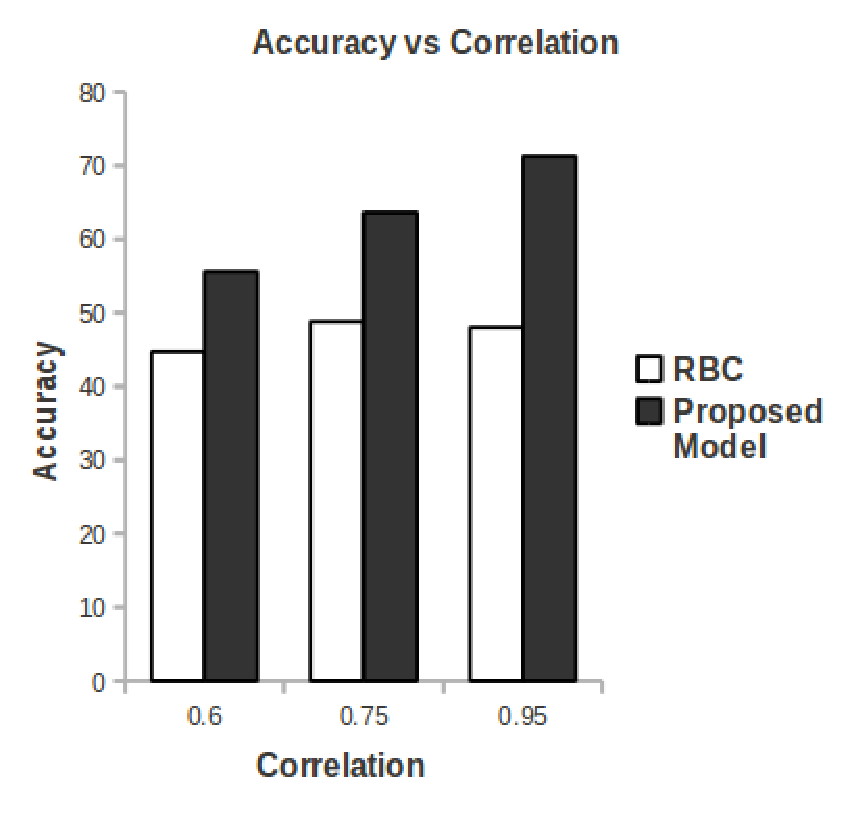
\includegraphics[scale=0.25]{/home/krishna/Desktop/Final7/shadi/img//acc-c.eps}
\label{fig:4.1}
\end{figure}
\end{block}
\column{0.5\textwidth} 
\begin{block}{Likelihood vs. Correlation}
\begin{figure}[htbp]
\centering
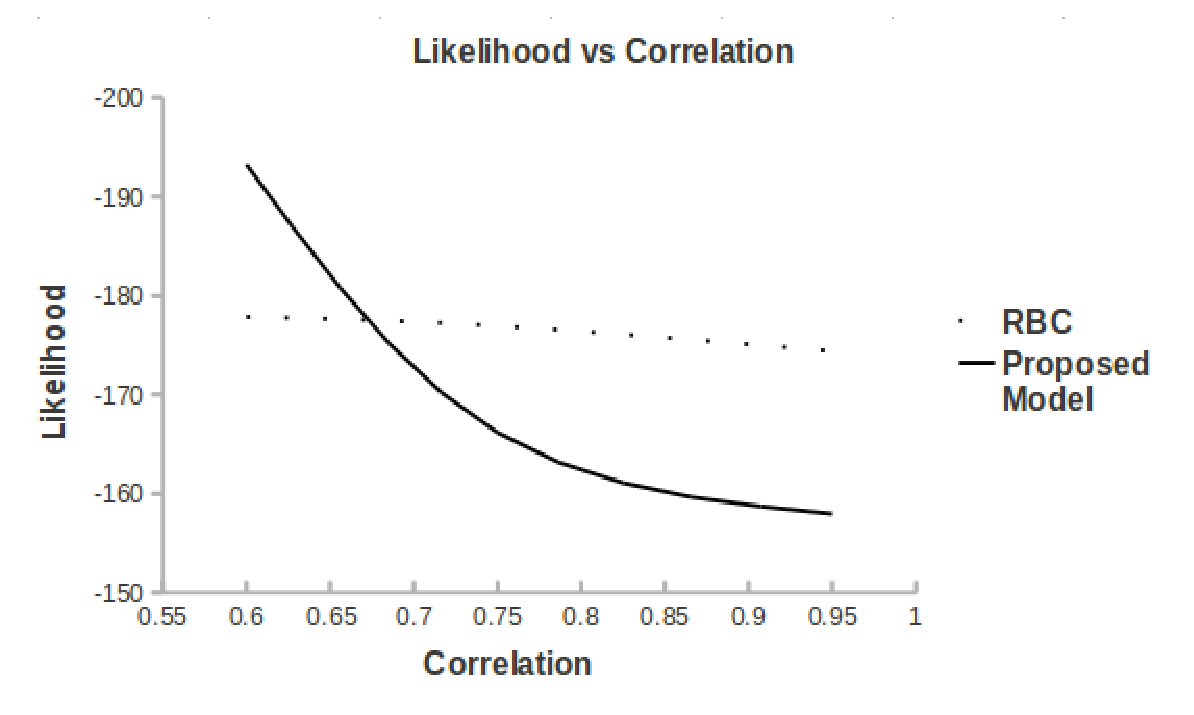
\includegraphics[scale=0.25]{/home/krishna/Desktop/Final7/shadi/img/lh-c.eps}
\label{fig:4.2}
\end{figure}
\end{block}
\end{columns}
\end{itemize}
Our model performs better than existing RBC in highly correlated environment
in both likelihood estimation as well as accuracy.
\end{frame}

\begin{frame}\frametitle{Synthetic Data Results}
\begin{itemize}
\item \textbf{Effect of Autocorrelation}
\begin{columns}[t]
\column{0.5\textwidth} 

\begin{block}{Accuracy vs. Autocorrelation}
\begin{figure}[htbp]
\centering
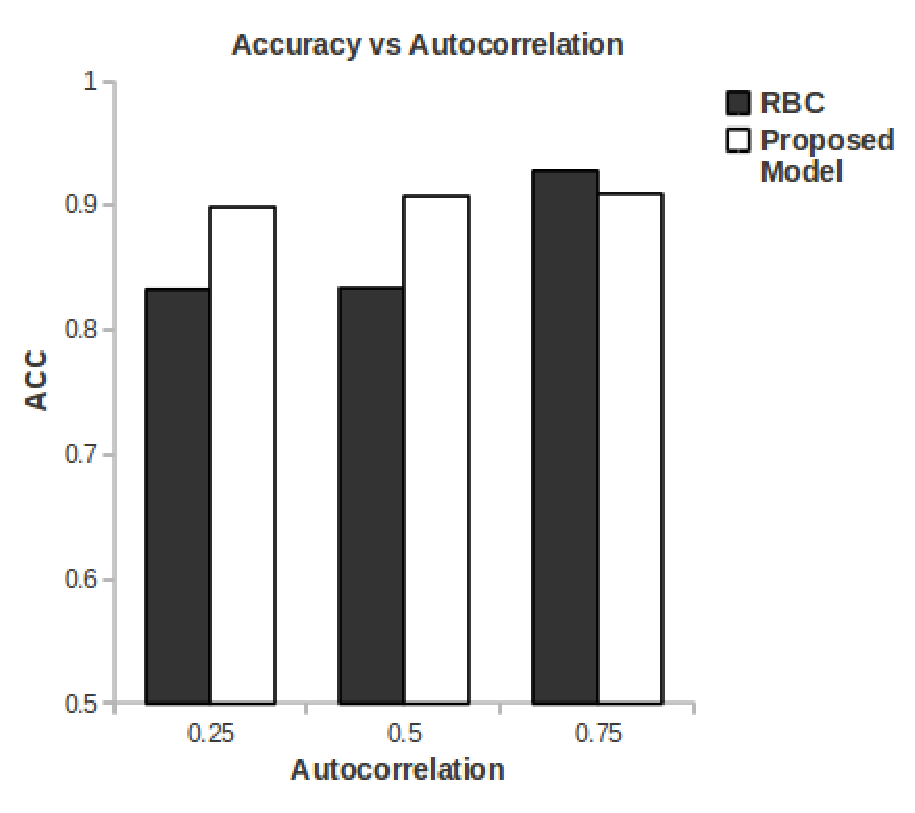
\includegraphics[scale=0.25]{/home/krishna/Desktop/Final7/shadi/img/acc-ac.eps}
\end{figure}
\end{block}

\column{0.5\textwidth} 

\begin{block}{Likelihood vs. Autocorrelation}
\begin{figure}[htbp]
\centering
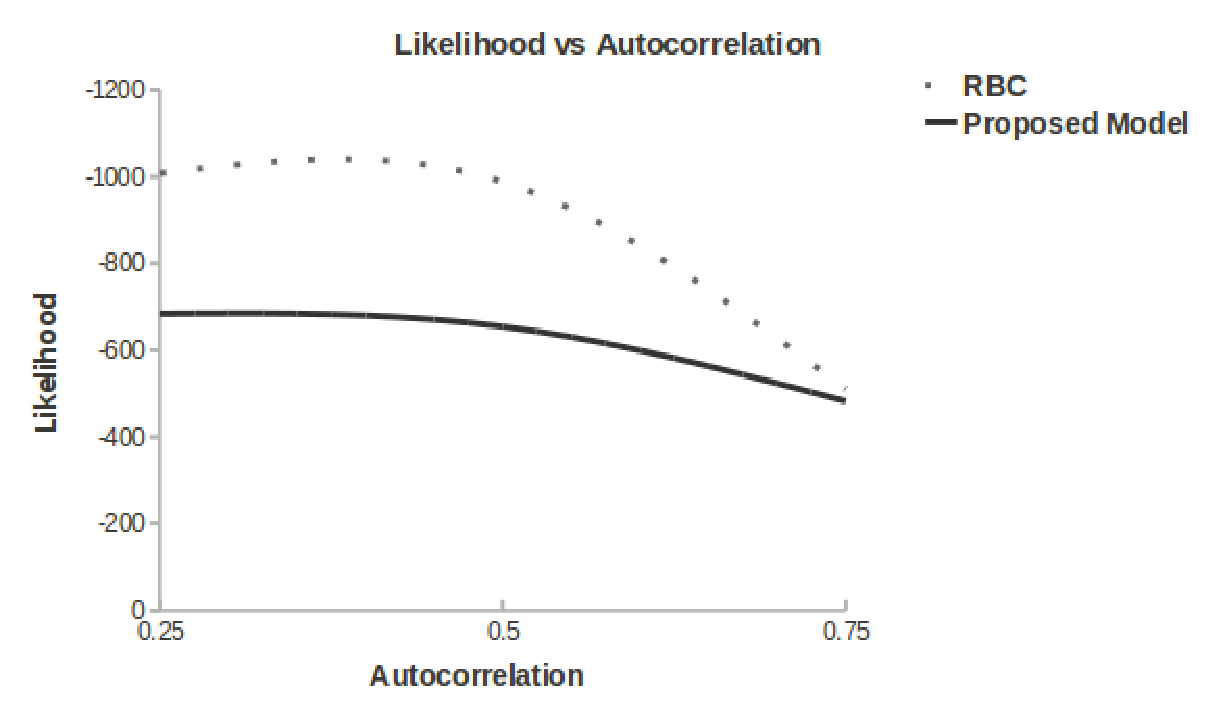
\includegraphics[scale=0.25]{/home/krishna/Desktop/Final7/shadi/img/lh-ac.eps}
\end{figure}

\end{block}
\end{columns}
\end{itemize}
\begin{itemize}
\item Performs better in low to moderate autocorrelation and comparable in high autocorrelation environment.
\item In high autocorrelation scenarios prediction is biased.
\end{itemize}
\end{frame}

\begin{frame}\frametitle{Synthetic Data Results}
\begin{itemize}
\item \textbf{Effect of Training Size}
\begin{columns}[t]
\column{0.5\textwidth} 

\begin{block}{Accuracy vs. Training Size}
\begin{figure}[htbp]
\centering
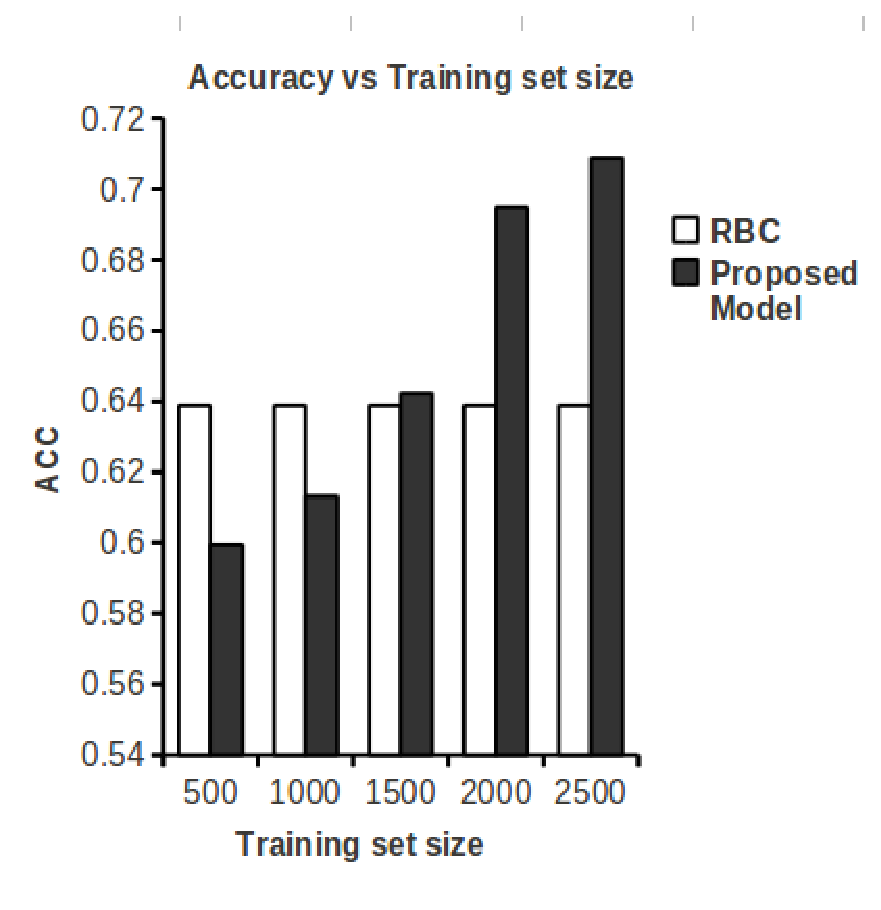
\includegraphics[scale=0.25]{/home/krishna/Desktop/Final7/shadi/img/acc-ts.eps}
\end{figure}
\end{block}

\column{0.5\textwidth} 

\begin{block}{Likelihood vs. Training Size}
\begin{figure}[htbp]
\centering
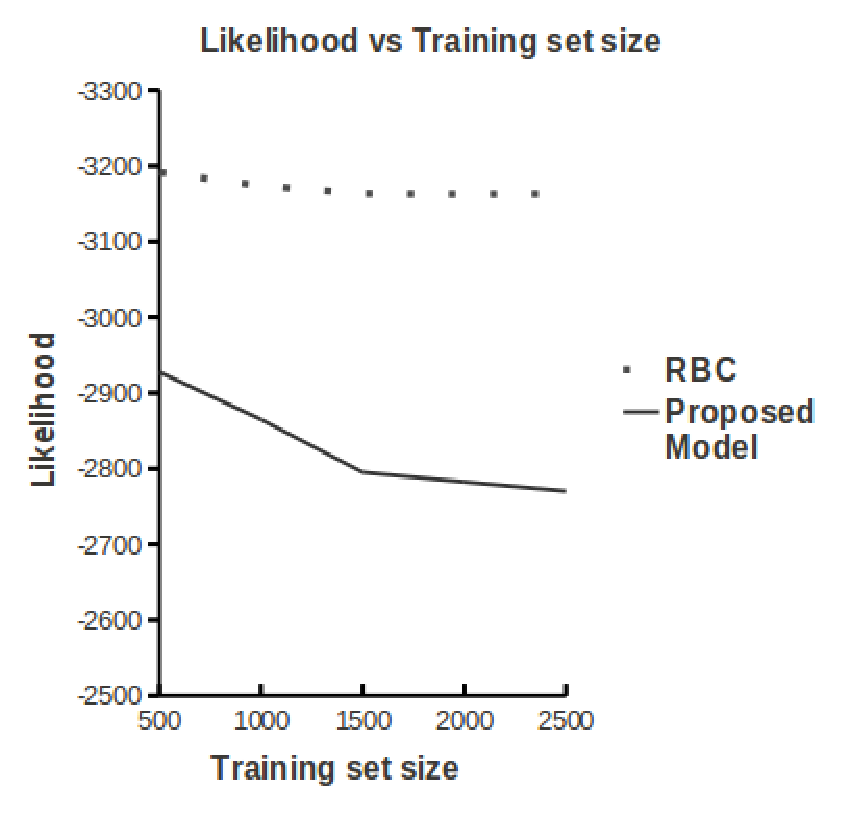
\includegraphics[scale=0.25]{/home/krishna/Desktop/Final7/shadi/img/lh-ts.eps}
\end{figure}

\end{block}
\end{columns}
\end{itemize}
\begin{itemize}
\item Second order RBC takes more training data to learn the high correlation present in the data.
\item Performs better than existing RBC in highly correlated environment
in both likelihood estimation as well as accuracy.
\end{itemize}
\end{frame}

\begin{frame}\frametitle{Real World Data Results}
\begin{block}{Experiments on three real world data sets}
\begin{itemize}
\item \textbf{HEP}
Predict the topic of paper given paper attributes, author names and
 publisher. 
 \item \textbf{MSN} Predict time stamp of mote to mote connections. 
 \item \textbf{ProxWebKB} Predict the category of a web page given it's linked page categories.
\end{itemize}
\end{block}
\begin{figure}[htbp]
\centering
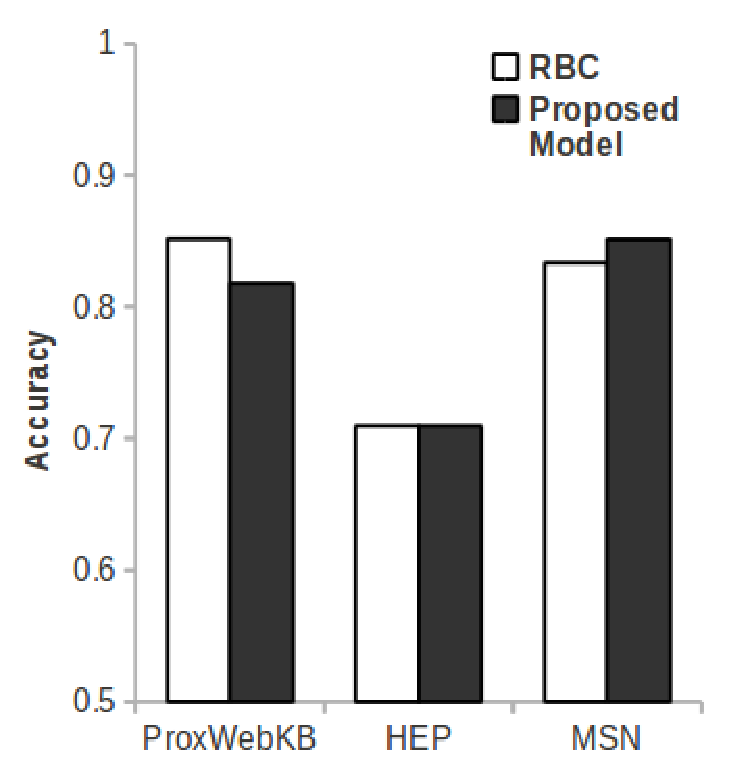
\includegraphics[scale=0.3]{/home/krishna/Desktop/Final7/shadi/img/model-acc.eps}
\end{figure}
\end{frame}

\begin{frame}\frametitle{HEP Data Set Result}

\begin{block}{Task}
We want to predict the \emph{``acceptability``} of a paper which is formed using paper citation degree and journal name.
\end{block}
\begin{columns}[t]
\column{0.5\textwidth} 

\begin{block}{Accuracy vs. Training Size}
\begin{figure}[htbp]
\centering
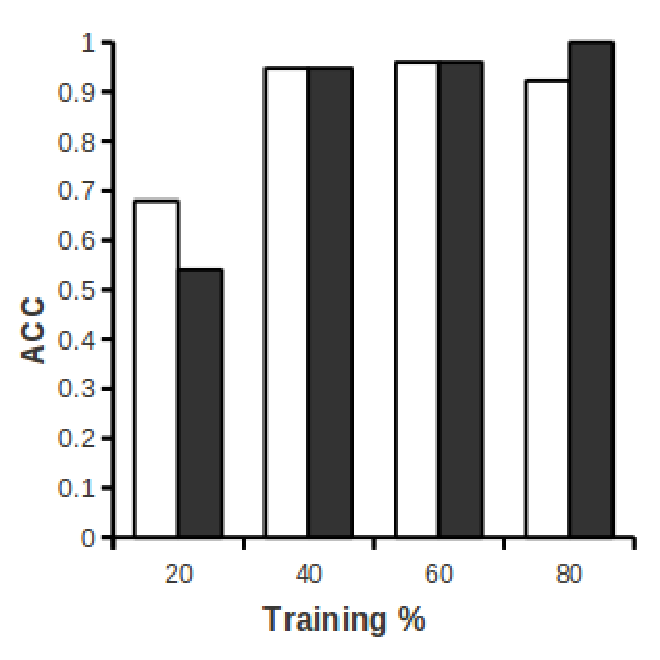
\includegraphics[scale=0.25]{/home/krishna/Desktop/Final7/shadi/img/hep-acc.eps}
\end{figure}
\end{block}

\column{0.5\textwidth} 

\begin{block}{Likelihood vs. Training Size}
\begin{figure}[htbp]
\centering
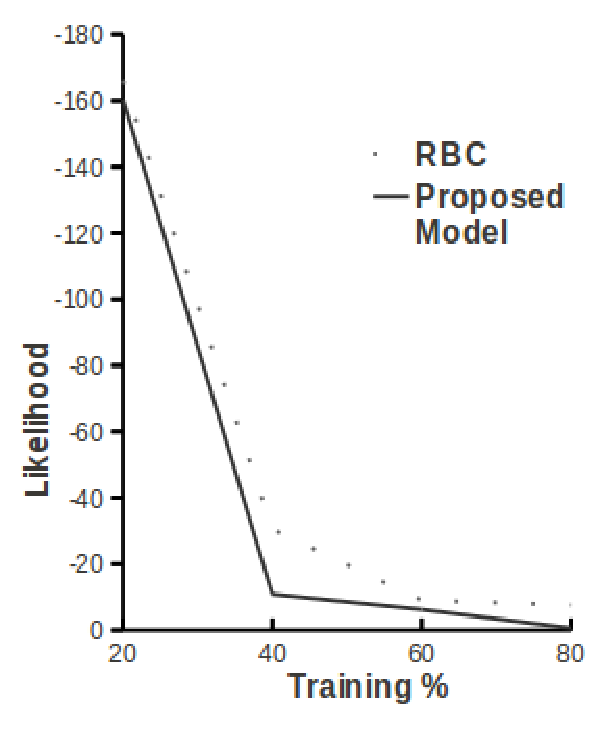
\includegraphics[scale=0.25]{/home/krishna/Desktop/Final7/shadi/img/hep-lh.eps}
\end{figure}
\end{block}
\end{columns}

\end{frame}

\section{Conclusion and Future Work}
\begin{frame}\frametitle{Conclusion and Future Work}
\begin{columns}[t]
\column{0.5\textwidth} 
\begin{flushleft}
\begin{block}{Conclusion}
\begin{itemize}
\item We demonstrated the use of second order pseudolikelihood in the RDN learning.
\item Extended RBC to second order setting.
\item Shown improvements in highly correlated data sets both in parameter estimation
and classification accuracy. 
\end{itemize}
\end{block}
\end{flushleft}
\column{0.5\textwidth} 
\begin{block}{Future Work}
\begin{itemize}
\item Making score function which will observe characteristic
of test subgraphs.
\item Selective models for Second order PL.
\item  Bias-variance analysis of the model.
\end{itemize}
\end{block}
\end{columns}
\begin{block}{}
\begin{center}
{\color{red}
ECML PKDD 2011!!}
\end{center}
\end{block}
\end{frame}


\begin{frame}
 
\begin{center}
\begin{figure}[htbp]
\centering
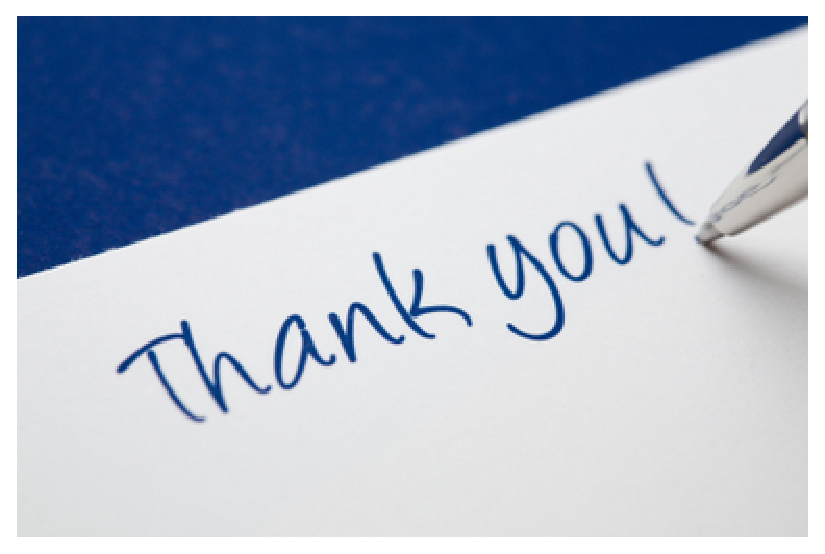
\includegraphics[scale=0.4]{/home/krishna/Desktop/Final7/shadi/img/222.eps}
\end{figure}
\end{center}
\end{frame} 


%-------------------------------------------------------------------------



\end{document}


